%%%%%%%%%%%%%%%%%%%%%%%%%%%%%%%%%%%%%%%%%
% fphw Assignment
% LaTeX Template
% Version 1.0 (27/04/2019)
%
% This template originates from:
% https://www.LaTeXTemplates.com
%
% Authors:
% Class by Felipe Portales-Oliva (f.portales.oliva@gmail.com) with template 
% content and modifications by Vel (vel@LaTeXTemplates.com)
%
% Template (this file) License:
% CC BY-NC-SA 3.0 (http://creativecommons.org/licenses/by-nc-sa/3.0/)
%
%%%%%%%%%%%%%%%%%%%%%%%%%%%%%%%%%%%%%%%%%

%----------------------------------------------------------------------------------------
%	PACKAGES AND OTHER DOCUMENT CONFIGURATIONS
%----------------------------------------------------------------------------------------

\documentclass[
	12pt, % Default font size, values between 10pt-12pt are allowed
%	UTF8
%	%letterpaper, % Uncomment for US letter paper size
	%spanish, % Uncomment for Spanish
]{fphw} %fphw
%\documentclass[12pt, UTF8]{ctexart}  %使用中文版的article文档类型排版,并选择UTF8编码格式

% Template-specific packages
\usepackage[UTF8]{ctex}	%使用ctex宏包,使得可以文中可以写中文
\usepackage[utf8]{inputenc} % Required for inputting international characters
\usepackage[T1]{fontenc} % Output font encoding for international characters
\usepackage{mathpazo} % Use the Palatino font

\usepackage{graphicx} % Required for including images
\usepackage{subfigure} %子图

\usepackage{booktabs} % Required for better horizontal rules in tables
\usepackage{listings} % Required for insertion of code
\usepackage{enumerate} % To modify the enumerate environment

%使得图片固定在某位置
\usepackage{float} 

%代码显示的包
\usepackage{listings}
\usepackage{xcolor}

%注释用
\usepackage{comment}
%----------------------------------------------
%配置代码显示格式-掌握minted之前的替代品
%----------------------------------------------
\definecolor{codegreen}{rgb}{0,0.6,0}
\definecolor{codegray}{rgb}{0.5,0.5,0.5}
\definecolor{codepurple}{rgb}{0.58,0,0.82}
\definecolor{backcolour}{rgb}{0.95,0.95,0.92}

\lstdefinestyle{mystyle}{
	backgroundcolor=\color{backcolour},   
	commentstyle=\color{codegreen},
	keywordstyle=\color{magenta},
	numberstyle=\tiny\color{codegray},
	stringstyle=\color{codepurple},
	basicstyle=\ttfamily\footnotesize,
	breakatwhitespace=false,         
	breaklines=true,                 
	captionpos=b,                    
	keepspaces=true,                 
	numbers=left,                    
	numbersep=5pt,                  
	showspaces=false,                
	showstringspaces=false,
	showtabs=false,                  
	tabsize=2
}

\lstset{style=mystyle}
%----------------------------------------------------------------------------------------


%----------------------------------------------------------------------------------------
%	ASSIGNMENT INFORMATION
%----------------------------------------------------------------------------------------

\title{第四章作业} % Assignment title

\author{MatthewNUST} % Student name

\date{October 18th, 2020} % Due date
%\date{\today}

\institute{深蓝学院 \\ 视觉SLAM} % Institute or school name

\class{视觉SLAM理论与实践} % Course or class name

\professor{高翔} % Professor or teacher in charge of the assignment

%----------------------------------------------------------------------------------------

\begin{document}

\maketitle % Output the assignment title, created automatically using the information in the custom commands above

%----------------------------------------------------------------------------------------
%	ASSIGNMENT CONTENT
%----------------------------------------------------------------------------------------

\section*{2.图像去畸变}

\begin{problem}
	请根据所给文件中内容,完成对该图像的去畸变操作。
\end{problem}
%\begin{center}
%	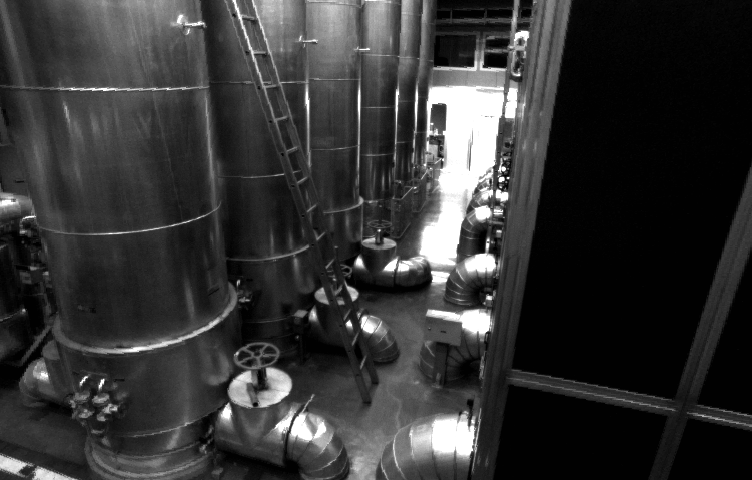
\includegraphics[width=0.5\columnwidth]{pic1.png} % Example image
%\end{center}
%pic
\begin{comment}
 \begin{figure}[h]
	\centering
	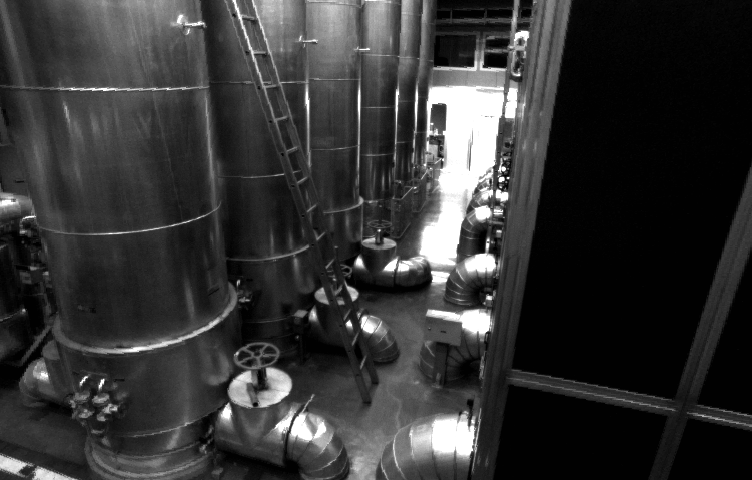
\includegraphics[width=0.5\columnwidth]{pic1.png} % Example image
	\caption{测试图像}
	\label{test_pic}
\end{figure}
\end{comment}
%------------------------------------------------

\subsection*{Answer}

基本思路是先将像素平面坐标变换到成像平面(归一化平面)上进行畸变纠正,纠正完毕后再变换回像素平面。添加的代码部分如下。
\begin{lstlisting}[language=C++, caption=题2所添代码]
	double x = (u-cx)/fx, y = (v - cy)/fy;	//变换到成像平面坐标系XOY
	double rpow2 = pow(x, 2) + pow(y, 2);
	double x_distorted = x*(1+k1*rpow2 + k2*rpow2*rpow2) + 2*p1*x*y + p2*(rpow2 + 2*x*x);
	double y_distorted = y*(1+k1*rpow2 + k2*rpow2*rpow2) + 2*p2*x*y + p1*(rpow2 + 2*y*y);
	u_distorted = fx * x_distorted + cx;
	v_distorted = fy * y_distorted + cy;	
\end{lstlisting}

得到的去畸变后的图像如图1(b)所示,与原图进行对比可知去畸变后图像在边缘存在一定损失。
\begin{figure}[ht]
	\centering
	\subfigure[测试图像]{               %小图题的名称
		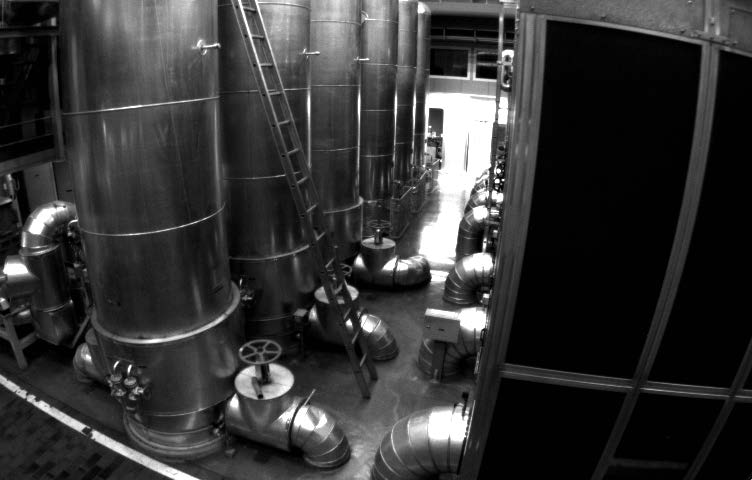
\includegraphics[width=7cm]{pic1.jpg}}
	\hspace{0in}
	\subfigure[去畸变后图像]{
		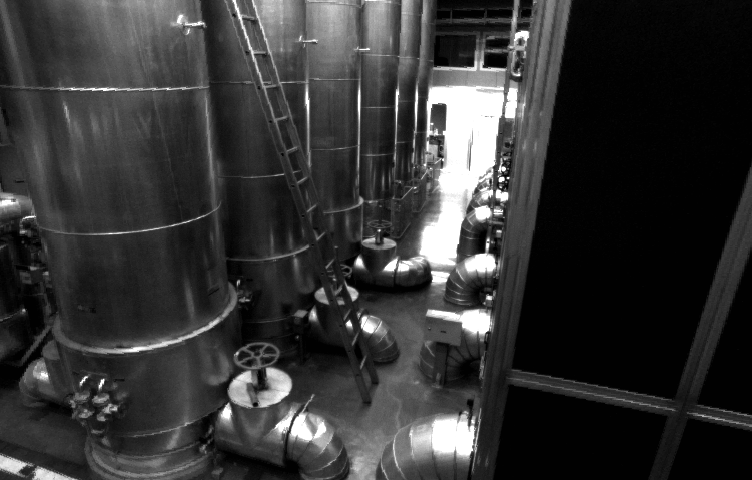
\includegraphics[width=7cm]{pic1_solved.png}}
	\caption{去畸变前后对比}
\end{figure}

%----------------------------------------------------------------------------------------
\clearpage
\section*{3.双目视差的使用}

\begin{problem}
	请根据给定参数,计算相机数据对应的点云,并显示到Pangolin 中。程序请参考code/disparity.cpp 文件。
	
	\medskip
	
%	\begin{enumerate}[(\itshape a\normalfont)] % Sub-questions styled as italic letters
%		\item Suppose ``chuck" implies throwing.
%		\item Suppose ``chuck" implies vomiting.
%	\end{enumerate}
\end{problem}

%------------------------------------------------

\subsection*{Answer}

在程序中添加上以下几行代码即可得到图2结果。

\begin{lstlisting}[language=C++, caption=题3所添代码]
	point[2] = fx*d/disparity.at<uchar>(v,u);
	point[0] = (u-cx)*point[2]/fx;
	point[1] = (v-cy)*point[2]/fy;
	pointcloud.push_back(point);	
\end{lstlisting}

值得注意的是此处得到的点云结果是基于left.png的(相当于直接将left.png这一像素平面坐标变换到成像平面并基于视差数据并添加上深度这一维度),所以disparity.cpp中并未对right.png进行有用的操作,那么我们也可以基于right.png文件进行相关操作。

\begin{figure}[h]
	\centering
	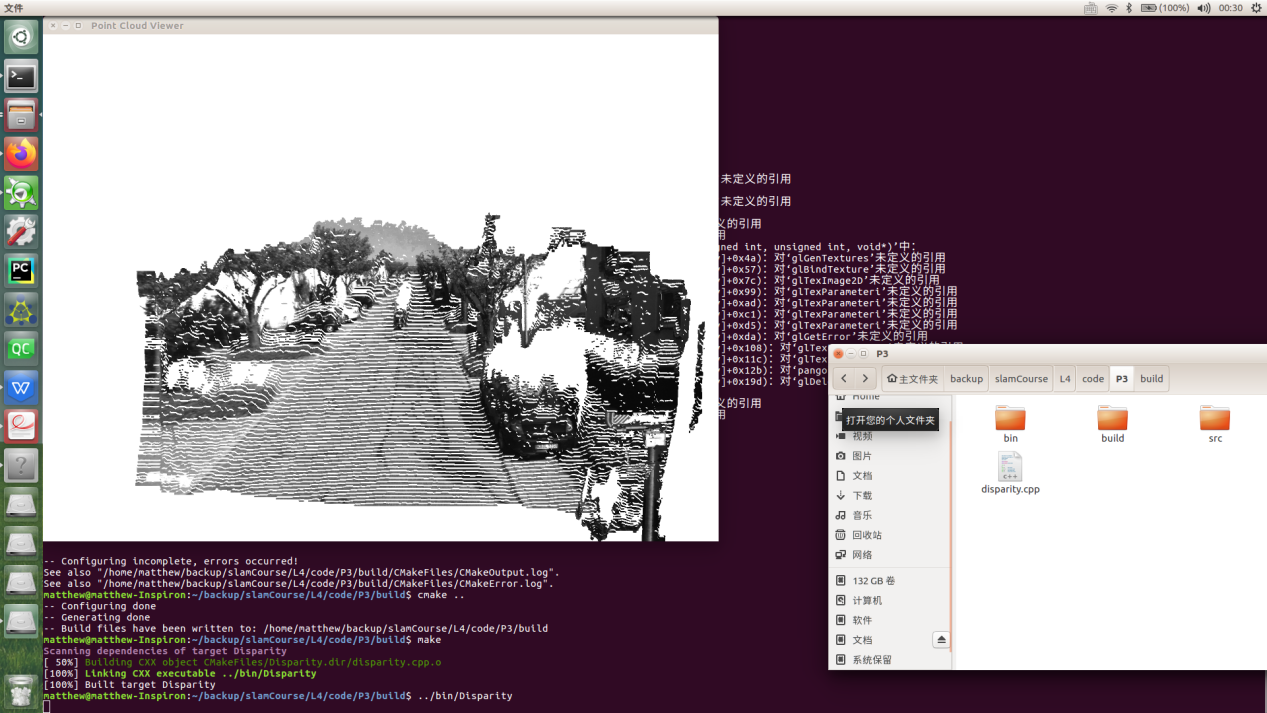
\includegraphics[width=0.9\columnwidth]{pic3.png} % Example image
	\caption{运行结果}
	%\label{test_pic}
\end{figure}

\begin{comment}
\begin{enumerate}[(\itshape a\normalfont)] % Sub-questions styled as italic letters
	\item According to the Associated Press (1988), a New York Fish and Wildlife technician named Richard Thomas calculated the volume of dirt in a typical 25--30 foot (7.6--9.1 m) long woodchuck burrow and had determined that if the woodchuck had moved an equivalent volume of wood, it could move ``about \textbf{700 pounds (320 kg)} on a good day, with the wind at his back".
    
	\item A woodchuck can ingest 361.92 cm\textsuperscript{3} (22.09 cu in) of wood per day. Assuming immediate expulsion on ingestion with a 5\% retainment rate, a woodchuck could chuck \textbf{343.82 cm\textsuperscript{3}} of wood per day.
\end{enumerate}
\end{comment}
%----------------------------------------------------------------------------------------
\clearpage
\section*{4.矩阵运算微分}

\begin{problem}
	设变量为$x\in R^N$,那么:
	\begin{enumerate}
		\item 矩阵$A\in R^{N\times N}$,那么d(Ax)/dx 是什么?
		\item 矩阵$A\in R^{N\times N}$,那么d(xTAx)/dx 是什么?
		\item 证明 $xTAx = tr(AxxT)$
	\end{enumerate}
	\medskip
\end{problem}

%------------------------------------------------

\subsection*{Answer} 

\begin{enumerate}
	\item 本题我采用的是原始定义证明法则。
	\begin{figure}[h]
		\centering
		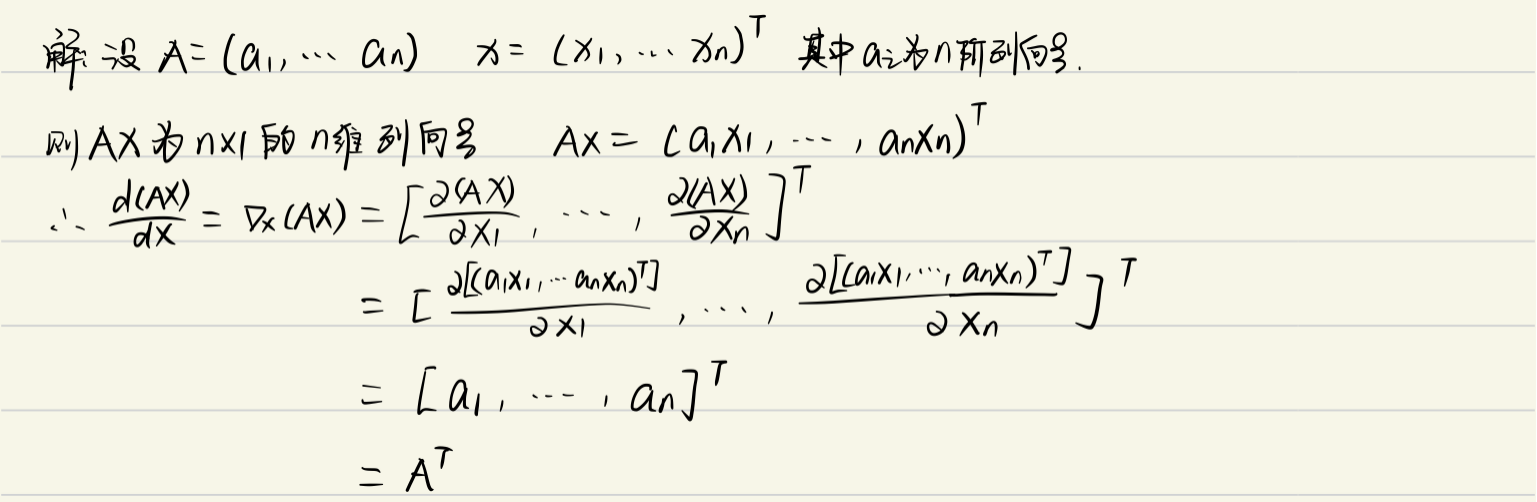
\includegraphics[width=1.0\columnwidth]{pic4_1.png} % Example image
		%\caption{运行结果}
		%\label{test_pic}
	\end{figure}
	\item 第一问使用了比较原始的证明方法,对于第二题而言证明过程会相当繁琐,所以在解答第二问之前我进一步查阅了相关资料\cite{matrix},了解到存在更为简便的求解方法\footnote{详见文献一p277。},下面使用此方法进行证明,为节省时间使用了书写版。
	\begin{figure}[H]
		\centering
		\includegraphics[width=1.0\columnwidth]{pic4_2.png} %  image
	\end{figure}
	\item 证明如下
	\begin{figure}[H]
		\centering
		\includegraphics[width=1.0\columnwidth]{pic4_3.png} %  image
	\end{figure}
\end{enumerate}

%----------------------------------------------------------------------------------------
\clearpage
\section*{5.高斯牛顿法的曲线拟合实验 (bonus marks)}

\begin{problem}
	现在请你书写Gauss-Newton的程序以解决此问题。程序框架见code/gaussnewton.cpp,请填写程序内容以完成作业
	
\begin{comment}
	\bigskip
    
	\begin{center}
		\begin{tabular}{l l l}
			\toprule
			\textit{Per 50g} & Pork & Soy \\
			\midrule
			Energy & 760kJ & 538kJ\\
			Protein & 7.0g & 9.3g\\
			Carbohydrate & 0.0g & 4.9g\\
			Fat & 16.8g & 9.1g\\
			Sodium & 0.4g & 0.4g\\
			Fibre & 0.0g & 1.4g\\
			\bottomrule
		\end{tabular}
	\end{center}
	
	\medskip
\end{comment}
\end{problem}

%------------------------------------------------

\subsection*{Answer}

所添加的第一处代码如下所示。Error代表第i个数据点的误差值,J[0]、J[1]、J[2]是error分别关于当前估计值对ae、be、ce的倒数。

\begin{lstlisting}[language=C++, caption=题5所添代码]
	double error;   // 第i个数据点的计算误差
	// 填写计算error的表达式
	error = yi - exp( ae * xi * xi + be * xi + ce );
	// 雅可比矩阵
	Vector3d J; 
	J[0] = - xi * xi * exp(ae * xi * xi + be * xi + ce);  // de/da
	J[1] = - xi * exp(ae * xi * xi + be * xi + ce);  // de/db
	J[2] = - exp(ae * xi * xi + be * xi + ce);  // de/dc
	
	H += J * J.transpose(); // GN近似的H
	b += -error * J;	
\end{lstlisting}

在求解线性方程时,由于H是雅各比矩阵乘以其自身的转置,故而H是一个SPD(实对称正定阵),联想到第二章所做的作业H可以进行比QR分解更为高效的Cholesky分解,因此使用Eigen的ldlt()函数进行计算(可见高博出的题还是很环环相扣的),代码为:
\begin{lstlisting}[language=C++, caption=题5所添代码] 
	Vector3d dx = H.ldlt().solve(b);
\end{lstlisting}
最后计算得到结果如图3所示,与所给参考答案一致。
\begin{figure}[h]
	\centering
	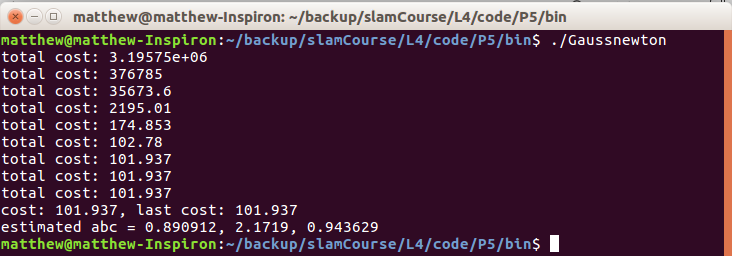
\includegraphics[width=0.8\columnwidth]{pic5.png} % Example image
	\caption{运行结果}
	%\label{test_pic}
\end{figure}

%----------------------------------------------------------------------------------------
\clearpage
\section*{6.* 批量最大似然估计}

\begin{problem}
	\begin{comment}
	\lstinputlisting[
		caption=Luftballons Perl Script, % Caption above the listing
		label=lst:luftballons, % Label for referencing this listing
		language=Perl, % Use Perl functions/syntax highlighting
		frame=single, % Frame around the code listing
		showstringspaces=false, % Don't put marks in string spaces
		numbers=left, % Line numbers on left
		numberstyle=\tiny, % Line numbers styling
	]{luftballons.pl}
\end{comment}
	\begin{enumerate}
		\item 可以定义矩阵H,使得批量误差为$e=z-Hx$。请给出此处H 的具体形式。
		\item 请给出此问题下W 的具体取值。
		\item 假设所有噪声相互无关,该问题存在唯一的解吗?若有,唯一解是什么?若没有,说明理由。
	\end{enumerate}

\end{problem}

%------------------------------------------------

\subsection*{Answer}

\begin{enumerate}
	\item 证明如下:
	\begin{figure}[H]
		\centering
		\includegraphics[width=1.0\columnwidth]{pic6_1.png} 
	\end{figure}
	\item 证明如下:
	\begin{figure}[H]
		\centering
		\includegraphics[width=1.0\columnwidth]{pic6_2.png} 
	\end{figure}
	\item 该问题存在唯一解,唯一解为对第二问最小二乘问题求解所得到的解。
\end{enumerate}

%----------------------------------------------------------------------------------------

%
\begin{thebibliography}{99}    %参考文献开始
	\bibitem{matrix}张贤达.矩阵分析与应用.清华大学出版社,2004.                    %参考文献1
	\bibitem{2}知乎."三步搞定矩阵求导".https:https://zhuanlan.zhihu.com/p/262751195.         %参考文献2
	\bibitem{3}CSDN."机器人所涉及的相关数学理论整理".https://blog.csdn.net/GFDYVJG/article/details/109121221.
	\bibitem{4}"Relationship between the Hessian and Covariance Matrix for Gaussian Random Variables".https://onlinelibrary.wiley.com/doi/pdf/10.1002/9780470824566.app1
\end{thebibliography}
\addcontentsline{toc}{section}{参考文献}


\end{document}
